    \documentclass[xcolor=x11names]{beamer}
%%%%%%%%%%%%%%%%%%%%%%%%%%%%%%%%%%%%%%%%%%%%%%%%%%%%%%%%%%%%
%%  This Beamer template was created by Cameron Bracken.
%%  Anyone can freely use or modify it for any purpose
%%  without attribution.
%%
%%  Last Modified by C. Bracken: January 9, 2009
%%
%%  The preamble, and maybe some modification of the Cameron Bracken's template is due to Attila Molnár.
%%
%%

%% General document
\usepackage[utf8]{inputenc}
\usepackage[T1]{fontenc}
\usepackage{graphicx}
\usepackage{tikz}
\usetikzlibrary{decorations.fractals}
\usetikzlibrary{decorations.text}
\usepgflibrary{arrows}
\usetikzlibrary{fadings}
\usetikzlibrary[decorations.pathmorphing]
\tikzfading[name=fade inside, inner color=transparent!70, outer color=transparent!70]
\usetikzlibrary{calc}
\usetikzlibrary{intersections}
\usetikzlibrary{shapes}
\usetikzlibrary{patterns}
\usefonttheme{serif}
\usepackage{amssymb} 			
\usepackage{amsmath}
\usepackage{ifthen}
\usepackage[normalem]{ulem}
\usepackage{mathrsfs}

%%%%%%%%%%%%%%%%%%%%%%%%%%%%%%%%%%%%%%%%%%%%%%%%%%%%%%%%%%%%%%%%%%%%%%%%%%%%%%%%%%%%
%% Beamer Layout %%%%%%%%%%%%%%%%%%%%%%%%%%%%%%%%%%
\useoutertheme[subsection=false,shadow]{miniframes}
\useinnertheme{default}
\usefonttheme{serif}
%\usepackage{txfonts} %Hook for strict implication!
\DeclareSymbolFont{symbolsC}{U}{txsyc}{m}{n}
\DeclareMathSymbol{\strictif}{\mathrel}{symbolsC}{74}
\DeclareMathSymbol{\boxright}{\mathrel}{symbolsC}{128}
\usepackage{palatino}
%\usepackage[uppercase=upright,charter]{mathdesign}

\setbeamerfont{title like}{shape=\scshape}
\setbeamerfont{frametitle}{shape=\scshape}


\setbeamercolor*{lower separation line head}{bg=white!40!DeepSkyBlue3}
\setbeamercolor*{normal text}{fg=black,bg=white}
\setbeamercolor*{alerted text}{fg=red}
\setbeamercolor*{example text}{fg=black}
\setbeamercolor*{structure}{fg=black}

\setbeamercolor*{palette tertiary}{fg=black,bg=white!90!DeepSkyBlue3}
\setbeamercolor*{palette quaternary}{fg=black,bg=black!10}

%\setbeamercolor{block body alerted}{bg=normal text.bg!90!DeepSkyBlue4}
\setbeamercolor{block body}{bg=normal text.bg!95!DeepSkyBlue3}
%\setbeamercolor{block body example}{bg=normal text.bg!90!DeepSkyBlue4}
%\setbeamercolor{block title alerted}{use={normal text,alerted text},fg=alerted text.fg!75!normal text.fg,bg=normal text.bg!90!DeepSkyBlue4}
\setbeamercolor{block title}{bg=normal text.bg!70!DeepSkyBlue3}
%\setbeamercolor{block title example}{use={normal text,example text},fg=example text.fg!75!normal text.fg,bg=normal text.bg!75!DeepSkyBlue4}

\setbeamertemplate{blocks}[rounded][shadow=true]
%\setbeamertemplate{background canvas}[vertical shading][bottom=white,top=structure.fg!25]
%\setbeamertemplate{sidebar canvas left}[horizontal shading][left=white!40!black,right=black]
\setbeamertemplate{itemize items}[circle]
\setbeamercolor*{itemize item}{fg=DeepSkyBlue3}
\setbeamercolor*{itemize subitem}{fg=DeepSkyBlue3}
\setbeamercolor*{itemize subsubitem}{fg=DeepSkyBlue3}
\setbeamertemplate{enumerate items}[circle]
%\setbeamercolor{item projected}{bg=DeepSkyBlue3,fg=black}
\setbeamercolor{item projected}{bg=white,fg=DeepSkyBlue3}
\setbeamercolor*{enumerate item}{fg=DeepSkyBlue3}
\setbeamercolor*{enumerate subitem}{fg=DeepSkyBlue3}
\setbeamercolor*{enumerate subsubitem}{fg=DeepSkyBlue3}

%%%%%%%%%%%%%%%%%%%%%%%%%%%%%%%%%%%%%%%%%%%%%%%%%%


%%%%%%%%%%%%%%%%%%%%%%%%%%%%%%%%%%%%%%%%%%%%%%%%%%%%%%%%%%%%%%%%%%%%%%%%%%%%%%%%%%%%

\newenvironment{defi}[1][]{\begin{block}{\footnotesize \textsc{Definition} \ifthenelse{\equal{#1}{}}{}{\, (#1)}}}{\end{block}}
\newenvironment{prop}[1][]{\begin{block}{\footnotesize \textsc{Proposition} \ifthenelse{\equal{#1}{}}{}{\, (\textsc{#1})}}}{\end{block}}
\newenvironment{lemm}[1][]{\begin{block}{\footnotesize \textsc{Lemma} \ifthenelse{\equal{#1}{}}{}{\, (\textsc{#1})}}}{\end{block}}
\newenvironment{idea}[1][]{\begin{block}{\footnotesize \textsc{Idea} \ifthenelse{\equal{#1}{}}{}{\, (\textsc{#1})}}}{\end{block}}
\newenvironment{rema}[1][]{\begin{block}{\footnotesize \textsc{Remark} \ifthenelse{\equal{#1}{}}{}{\, (\textsc{#1})}}}{\end{block}}
\newenvironment{coro}[1][]{\begin{block}{\footnotesize \textsc{Corollary} \ifthenelse{\equal{#1}{}}{}{\, (\textsc{#1})}}}{\end{block}}
\newenvironment{tete}[1][]{\begin{block}{\footnotesize \textsc{Theorem} \ifthenelse{\equal{#1}{}}{}{\, (\textsc{#1})}}}{\end{block}}
\newenvironment{claim}[1][]{\begin{block}{Claim \ifthenelse{\equal{#1}{}}{}{\, (\textsc{#1})}}}{\end{block}}
%\newenvironment{lemma}[1][]{\begin{block}{Lemma \ifthenelse{\equal{#1}{}}{}{\, (\textsc{#1})}}}{\end{block}}
\newenvironment{question}[1][]{\begin{block}{Question \ifthenelse{\equal{#1}{}}{}{\, (\textsc{#1})}}}{\end{block}}
\newenvironment{rem}[1][]{\begin{block}{Remark \ifthenelse{\equal{#1}{}}{}{\, (\textsc{#1})}}}{\end{block}}
\newenvironment{homework}[1][]{\begin{block}{Homework \ifthenelse{\equal{#1}{}}{}{\, (\textsc{#1})}}}{\end{block}}
\newenvironment{proo}[1][]{\begin{block}{\footnotesize \textsc{Proof} \ifthenelse{\equal{#1}{}}{}{\, (\textsc{#1})}}}{\end{block}}

%%%%%%%%%%%%%%%%%%%%%
%% To evade unnecessary circles, mainly for \cimdia
%%%%%%%%%%%%%%%%%%%%%

\makeatletter
\let\beamer@writeslidentry@miniframeson=\beamer@writeslidentry
\def\beamer@writeslidentry@miniframesoff{%
  \expandafter\beamer@ifempty\expandafter{\beamer@framestartpage}{}% does not happen normally
  {%else
    % removed \addtocontents commands
    \clearpage\beamer@notesactions%
  }
}
\newcommand*{\miniframeson}{\let\beamer@writeslidentry=\beamer@writeslidentry@miniframeson}
\newcommand*{\miniframesoff}{\let\beamer@writeslidentry=\beamer@writeslidentry@miniframesoff}
\makeatother

%%%%%%%%%%%%%%%%%%%%%%%%%%%%%
%%%%%%%%%%%%% END %%%%%%%%%%%
%%%%%%%%%%%%%%%%%%%%%%%%%%%%%


%%%% Formatting Commands

\newcommand{\cimdia}[1] {\miniframesoff \begin{frame}\begin{center}\huge \begin{tabular}{c}#1\end{tabular}\end{center}\end{frame}\miniframeson}
\newcommand{\szakasz}[2][]{\section{#1}\subsection{}\cimdia{#2}}
\newcommand{\bluebullet}{\textcolor{DeepSkyBlue3}{\quad $\bullet$} \,\,}

\newenvironment{frame*}[1][]{\miniframesoff \begin{frame} #1}{\end{frame}\miniframeson}

  % for admissible intersections
  \newcommand{\bigsqcap}{\rotatebox[origin=c]{180}{$\bigsqcup$}}

\newcommand{\felkorvonal}[2]{\draw[rounded corners=0] (180+#1:.25*#2 cm) arc (180+#1:360+#1:.25*#2 cm)--cycle;}
\newcommand{\pecset}[2]{\begin{tikzpicture}[remember picture,overlay]
\node [ draw=red, rectangle, rounded corners=5mm, inner sep=1mm, ultra thick, fill=white, fill opacity=.8, rotate=30, scale=#1, text opacity=0.7] at (current page.center) {#2};\end{tikzpicture}}

\newcommand{\felirat}[7][]{\begin{tikzpicture}[remember picture,overlay]
\node [draw=DeepSkyBlue3, rectangle, rounded corners=#3 mm, inner sep=#2mm, ultra thick, fill=white, fill opacity=.8, scale=#4, text opacity=1,#1]
at ([xshift=#5 cm, yshift=#6 cm]current page.center) {#7};
\end{tikzpicture}}

\newcommand{\hazi}[6]{\begin{tikzpicture}[remember picture,overlay]
\node [ draw=Coral1,
        rectangle,
        rounded corners=#2 mm,
        inner sep=#1mm,
        ultra thick,
        fill=white,
        fill opacity=.8,
        rotate=0,
        scale=#3,
        text opacity=1]
        at ([xshift=#4 cm, yshift=#5 cm]current page.center)
        {#6};
\end{tikzpicture}}

\newcommand{\underconstruction}[1]{\begin{tikzpicture}[remember picture,overlay]
\node [rectangle, rounded corners=5mm, inner sep=1mm, rotate=30, scale=#1, text opacity=0.4]at (current page.center){\textsc{\textcolor{orange}{\begin{tabular}{c}under \\construction\end{tabular}}}};
\end{tikzpicture}}

\newcommand{\dzsa}[1]{\textsc{\underline{#1}}:}
\newcommand{\axiom}[1]{\bemph{(\mathrm{#1})}}



% Emphasizing:
\definecolor{barna}{rgb}{0.5,0.2,0.1}
\newcommand{\bemph}[1] {{\color{DeepSkyBlue3}{#1}}}
\newcommand{\kemph}[1] {{\color{blue}{#1}}}
\newcommand{\cemph}[1]{\textcolor{red}{#1}}
\newcommand{\zemph}[1] {{\color{Green2}{#1}}}
\newcommand{\yemph}[1] {{\color{Orange1}{#1}}}
%\renewcommand{\emph}[1]{\textbf{#1}}

\newcommand{\FD}{\mathbf F}
\newcommand{\FB}{\mathbf G}
\newcommand{\PD}{\mathbf P}
\newcommand{\PB}{\mathbf H}
\newcommand{\GB}{\mathbf A}
\newcommand{\GD}{\mathbf E}

\newcommand{\Pmodels}{\mathrel{\models \hspace{-1.8ex} \raisebox{1.1ex}{\scalebox{.5}{$\mathrm{\bemph{P}}$}} }\,}
\newcommand{\Omodels}{\mathrel{\models \hspace{-1.8ex} \raisebox{1.1ex}{\scalebox{.5}{$\mathrm{\bemph{O}}$}} }\,}
\newcommand{\Kmodels}{\mathrel{\models \hspace{-1.8ex} \raisebox{1.1ex}{\scalebox{.5}{$\mathrm{\bemph{K}}$}} }\,}
\newcommand{\Bmodels}{\mathrel{\models \hspace{-1.8ex} \raisebox{1.1ex}{\scalebox{.5}{$\mathrm{\bemph{B}}$}} }\,}
\newcommand{\tru}{\textup{true}}
\newcommand{\fal}{\textup{false}}
\newcommand{\und}{\textup{undefined}}


\newcommand{\FDDot}{\underline{\mathbf F}}
\newcommand{\FBDot}{\underline{\mathbf G}}
\newcommand{\PDDot}{\underline{\mathbf P}}
\newcommand{\PBDot}{\underline{\mathbf H}}

\newcommand{\CFD}{\mathbf F^c}
\newcommand{\CFB}{\mathbf G^c}
\newcommand{\CPD}{\mathbf P^c}
\newcommand{\CPB}{\mathbf H^c}

\newcommand{\CFDDot}{\underline{\mathbf F^c}}
\newcommand{\CFBDot}{\underline{\mathbf G^c}}
\newcommand{\CPDDot}{\underline{\mathbf P^c}}
\newcommand{\CPBDot}{\underline{\mathbf H^c}}

\renewcommand{\Diamond}{\scalebox{.9}{\raisebox{-.4ex}{\rotatebox{45}{$\Box$}}}}

%causal
\newcommand{\past}{\succ}
\newcommand{\pasteq}{\succeq}
\newcommand{\future}{\prec}
\newcommand{\futureeq}{\preceq}
%lightlike
\newcommand{\llpast}{\nwarrow}
\newcommand{\llpasteq}{\underline\nwarrow}
\newcommand{\llfuture}{\nearrow}
\newcommand{\llfutureeq}{\mathop{\underline\nearrow}}
%timelike
\newcommand{\tlpast}{\gg}
\newcommand{\tlpasteq}{\underline \gg}
\newcommand{\tlfuture}{\ll}
\newcommand{\tlfutureeq}{\underline \ll}

\newcommand{\egyuttjar}{\mathop{\uparrow \uparrow}}
\newcommand{\Between}{\mathrm{B}}
\newcommand{\EqDist}{\equiv}
\newcommand{\ISCM}{\uparrow\equiv\uparrow}

 \newcommand{\vonal} [1][.2]{\hspace{#1cm} | \hspace{#1cm}}

 \newcommand{\lrule}[3][c]{\begin{array}{#1} #2  \\  \hline #3 \end{array}}
 \newcommand{\dlrule}[3][c]{\begin{array}{#1} #2  \\  \hline\hline #3 \end{array}}
 \newcommand{\dual}{\delta}

 \newcommand{\mono}{\rightarrowtail}
 \newcommand{\epi}{\twoheadrightarrow}
 \newcommand{\iso}{\rightarrowtail \!\!\!\!\! \rightarrow}

 \newcommand{\defegy}[1][.1]{\hspace{#1cm}\overset{\textup{\tiny def}}{=}\hspace{#1cm}}
 \newcommand{\defpont}[1][.1]{\hspace{#1cm}\overset{\textup{\tiny def}}{:}\hspace{#1cm}}
 \newcommand{\defekv}[1][.1]{\hspace{#1cm}\overset{\textup{\tiny def}}{ \Leftrightarrow }\hspace{#1cm}}
 \newcommand{\lthen}{\rightarrow}
 \newcommand{\liff}{\leftrightarrow}
 \newcommand{\forallin}[2]{(\forall #1 \in #2)}
 \newcommand{\existsin}[2]{(\exists #1 \in #2)}
 \newcommand{\nexistsin}[2]{(\nexists #1 \in #2)}
 \newcommand{\forallp}[1]{(\forall #1)}
 \newcommand{\existsp}[1]{(\exists #1)}

 \newcommand{\points}[1][0]{\hspace{#1ex}\hspace{-.5ex}:\hspace{-.5ex}\hspace{#1ex}}
 \newcommand{\Points}{\mathrm{P}}
 \newcommand{\Pointsf}{\mathrm{p}}
 \newcommand{\Ex}{\mathrm{E}}

\newcommand{\wline}[1]{\mathrm{wline}_{#1}}

\newcommand{\magyi}[1]{\textup{\bemph{\tiny #1}}}
\newcommand{\magyarazat}[2]{\overset{\substack{\textup{#2}\\ \downarrow}}{#1}}
\newcommand{\wintension}[3][]{{[}\hspace{-.46mm}{[} {#3}{]}\hspace{-.46mm}{]}^{\mathfrak{#1}}_{#2}}
\newcommand{\canintension}[2][]{{[}\hspace{-.46mm}{[} {#2}{]}\hspace{-.46mm}{]}_{\mathrm{#1}}}
\newcommand{\intension}[2][]{{[}\hspace{-.46mm}{[} {#2}{]}\hspace{-.46mm}{]}^{\mathfrak{#1}}}

\newcommand{\theory}[2][]{\mathrm{th}_{\mathfrak{#1}}(#2)}

\newcommand{\seenby}{\reflectbox {$R$}}
\newcommand{\derives}[1][]{\vdash_{\mathrm{#1}}}


\newcommand{\PBTemplate}[1]{{#1} \overrightarrow {\PB}}
\newcommand{\FBTemplate}[1]{{#1} \overrightarrow {\FB}}
\newcommand{\BoxTemplate}[1]{{#1} \overrightarrow {\Box}}
\newcommand{\PDTemplate}[1]{{#1} \widehat {\PD}}
\newcommand{\FDTemplate}[1]{{#1} \widehat {\FD}}
%\newcommand{\DiamondTemplate}[1]{#1\hspace{-.2ex} \mathop{\Diamond\hspace{-1.35ex} \raisebox{.4ex}{\scalebox{.5}{$\land$}}}\,}

%%%%%%%%%%%%%%%%%%%%%%%%%%%%%%%%%%%%%%%%%%%%%%%%%%%%%%
\newenvironment{tomb}[2][.1]{\arraycolsep=#1cm\begin{array}{#2}}{\end{array}}

\beamertemplatenavigationsymbolsempty


\author{Attila Moln\'ar}
\date{2014. March 21.}
\title{Test}
\institute{ELTE}
\begin{document}
\footnotesize


\szakasz[Ockhamist axioms]{Ockhamist axioms}

\begin{frame}[t]
\frametitle{$\mathbf O:$% \defegy \mathbf{K4.3}_{\FD, \PD} + \mathbf{S5}_{\scalebox{.7}{\Diamond}}$} %= \mathbf K.3_{\FD,\PD} + \mathbf S5_\Diamond + (IRR)+(UPP)+(WDC1)+(WDC2)+(MB)$}
%\framesubtitle{
%Logic of Kamp-frames and
Ockhamist bundled trees}
\scriptsize
\begin{minipage}[t]{5.78cm}
$\mathbf{PC}$: {Classical logic}
\begin{itemize}
\item[(PC1)] $\varphi \lthen .\psi \lthen \varphi$
\item[(PC2)] $\varphi\lthen (\psi \lthen \chi) \lthen\!\!. (\varphi \lthen \psi) \lthen\!\! . \varphi \lthen \chi$
\item[(PC3)] $\varphi \lthen \psi \lthen .\lnot \psi \lthen \lnot \varphi$
\item[(MP)] $\lrule {\varphi , \; \varphi \lthen \psi}{\psi}$
\end{itemize}
\pause %%%%%%%%%%%%%%%%%%%%%% PAUSE %%%%%%%%%%%%%%%%%%%%%%%
\bemph{\hrule}
\smallskip

$\mathbf{K4.3_{\FD, \PD}}$: {Temporal logic of linear frames}
\begin{itemize}
\item[(A)] $(\FB\varphi \land \FB \psi )\lthen \FB(\varphi \land \psi )$,\quad  $(\PB\varphi \land \PB \psi )\lthen \PB(\varphi \land \psi )$
\item[(Lem)] $\lrule{\varphi\lthen \psi}{\PB\varphi \lthen \PB\psi}$, \quad $\lrule{\varphi\lthen \psi}{\FB\varphi \lthen \FB\psi}$
\item[(C)] $\PD\FB\varphi \lthen \varphi $, \quad  $\FD\PB\varphi \lthen \varphi$
\item[(4)] $\FB\varphi\lthen \FB\FB\varphi$
\item[(.3)] $\PB(\PBDot \varphi\lthen \psi ) \lor \PB(\PBDot \psi\lthen \varphi )$, \quad $\FB(\FBDot \varphi\lthen \psi ) \lor \FB(\FBDot \psi\lthen \varphi )$
\end{itemize}
\pause %%%%%%%%%%%%%%%%%%%%%% PAUSE %%%%%%%%%%%%%%%%%%%%%%%
\bemph{\hrule}
\smallskip
Irreflexivity rule:
\begin{itemize}
\item[(IRR)] $\lrule{(p\land \mathbf H \lnot p) \lthen \varphi}{\varphi}$  \textup{\tiny where $p$ does not occur in $\varphi$}
\end{itemize}
\end{minipage}\quad
\begin{minipage}[t]{4.7cm}
\pause
$\mathbf{S5}_{\Diamond}$: {Alethic
logic of equiv. relations}
\begin{itemize}
\item[(A)] $(\Box\varphi \land \Box \psi )\lthen \Box(\varphi \land \psi )$
\item[(Lem)] $\lrule{\varphi\lthen \psi}{\Box\varphi \lthen \Box\psi}$
\item[(T)] $\Box \varphi \lthen \varphi$
\item[(4)] $\Box \varphi\lthen \Box \Box \varphi$
\item[(B)] $\Diamond \Box \varphi \lthen \varphi$
\end{itemize}
\pause %%%%%%%%%%%%%%%%%%%%%% PAUSE %%%%%%%%%%%%%%%%%%%%%%%
\bemph{\hrule}
\smallskip
Full-blooded Ockhamist axioms
\begin{itemize}
\item[(UPP)] $ \varphi \lthen \Box \varphi $ {\tiny where $\FD $ does not occur in $\varphi$}.\\ \hfill \magyi{unpreventability of past}
\item[(WDC)] $ \varphi\lthen \FB \Box \PD \Diamond \varphi$ \\ \hfill \magyi{weak diagram completion}
\item[(WDC+)]$ (p \land \PB \lnot p \land \Box \varphi) \lthen $ \\ \hfill $\lthen \FB \Box \PB ((p \land \PB \lnot p) \lthen \varphi)$
\item[(MB)]  $ \FB \bot \lthen \Box \FB \bot $ \hfill \magyi{maximality of branches}
\end{itemize}
\end{minipage}
\end{frame}
%%%%%%%%%%%%%%%%%%%%%%%%%%%%%%%%%%%%%%%%%%%%%%%%%%%%%%%%%%%%%%%%%%%%%%%%%%
\begin{frame}[t]
	\frametitle{IRR-rule}
\scriptsize
\dzsa{Lemma} The IRR rule is valid:
\[(IRR) \qquad \lrule{(p\land \mathbf H \lnot p) \lthen \varphi}{\varphi} \qquad \textup{ where $p$ does not occur in $\varphi$}\]
\hrule
\medskip
\dzsa{Proof} Suppose that $(p\land \mathbf H \lnot p) \lthen \varphi$ is valid on a \cemph{Kamp-frame} $\mathfrak K$, i.e., true in all worlds w.r.t. any Kamp-valuation. Now take an arbitrary but fixed world $w$ and Kamp-valuation $V$. We will prove that $\mathfrak K, V, w \Kmodels \varphi $
%Let $V'$ be
%\[ V'\defegy V[p\mapsto \{v \, : \, w\equiv v\}] \]
%Note that by that -- since the model is a Kamp-model! -- we have that $\mathfrak K, V', w \Kmodels p\land \mathbf H\lnot p$.
%To sum up:
\[\begin{tomb}{rcll}
   \mathfrak K, V[p\mapsto \{v : w\equiv v\}], w &\Kmodels &(p\land \mathbf H \lnot p) \lthen \varphi&  \magyi{assumption}
\\ \mathfrak K, V[p\mapsto \{v : w\equiv v\}], w &\Kmodels & p\land \mathbf H \lnot p &  \magyi{By $V[p\mapsto \{v : w\equiv v\}]$}
\\ \mathfrak K, V[p\mapsto \{v : w\equiv v\}], w &\Kmodels &\varphi &  \magyi{modus ponens}
\\ \mathfrak K, V, w &\Kmodels &\varphi &  \magyi{$p$ did not occur in $\varphi$}
\end{tomb}\]

\vspace{-2em}

\hfill $\blacksquare$
\end{frame}
%%%%%%%%%%%%%%%%%5%%%%%%%%%%%%%%%%%5%%%%%%%%%%%%%%%%%5%%%%%%%%%%%%%%%%%5%%%%%%%%%%%%%%%%%5%%%%%%%%%%%%%%%%%5
\begin{frame}[t]
	\frametitle{Completeness Plan}
\tiny
\begin{enumerate}\tiny
\item  We construct an \cemph{irreflexive} submodel $\mathfrak M_{\mathbf O}^{\mathrm{IRR}}$ of the canonical Kamp model $\mathfrak M_{\mathbf O}$. We will prove that we can use that model to prove a completeness proof. $W_{\mathbf O}^{\mathrm{IRR}}$ will be those maximally $\mathbf O$-consistent worlds that are at the same time \emph{IRR theories}, which we will define later, but in the meantime, the following properties will show why do we focus on that property:
\begin{enumerate}\tiny
\item[irr.] If $\Gamma$ is a maximally ${\mathbf{O}}$-consistent IRR theory, then it is not true that $\Gamma <_\mathbf{O}\Gamma$.
\item[cl.irr.] If $\Gamma$ is a maximally ${\mathbf{O}}$-consistent IRR theory, then there is no maximally ${\mathbf{O}}$-consistent IRR theory $\Gamma'$ s.t. $\Gamma <_\mathbf{O}\Gamma'$ and $\Gamma \equiv_\mathbf{O}\Gamma$.
\item[(IRRExt)] If $\Gamma$ is ${\mathbf{O}}$-consistent and \bemph{an infinite number of atomic sentences does not occur in $\Gamma$}, then it can be extended into an ${\mathbf{O}}$-consistent IRR theory $\Gamma^+$.
\item[(IRRLin)] If $\Gamma$ is ${\mathbf{O}}$-consistent and IRR, then it can be extended into maximally ${\mathbf{O}}$-consistent IRR theory $\Gamma^+$.
\item[$(\mathrm L^-)$] If $\Gamma$ is IRR, then so is $\mathrm{L}^-(\Gamma)$ for any $\mathrm{L}\in \{\Box , \FD, \PB\}$.
\item[(FE)] If $\Gamma$ is IRR, then so is $\Gamma\cup \{\varphi\}$ for any $\varphi\in \mathcal L_{\mathbf {O}}$.
\item[(Ex)] If $\Gamma$ is an max. ${\mathbf{O}}$-con. IRR theory s.t. $\Diamond \varphi \in \Gamma$, then there is a $\Gamma'$ s.t. $\Gamma R_{\mathbf O} \Gamma'$ and $\varphi \in \Gamma'$, where $R_{\mathbf{O}}\in \{<_\mathbf O, \equiv_{\mathbf O} \}$.
\item[(Truth)] Truth is membership in the IRR submodel of the canonical model.
\item[($\mathrm{CMT}^-$)] The IRR submodel of the canonical model is \cemph{almost} a Kamp model -- canonicity proofs for all property except the maximality of histories.
\end{enumerate}
\item We transform $\mathfrak M_{\mathbf{O}}^{\mathrm{IRR}}$ into an $\mathrm {MB}(\mathfrak M_{\mathbf{O}}^{\mathrm{IRR}})$ in which the histories are maximal.
\item We prove that $\mathfrak M_{\mathbf{O}}^{\mathrm{IRR}}$ is a zigzag image of $\mathrm {MB}(\mathfrak M_{\mathbf{O}}^{\mathrm{IRR}})$.
\\ \magyi{We can conclude a weak completeness theorem for Kamp semantics}
\item We construct a bundled tree model $\mathrm{BT}(\mathrm {MB}(\mathfrak M_{\mathbf{O}}^{\mathrm{IRR}}))$ which satisfy the same formulas as $\mathrm {MB}(\mathfrak M_{\mathbf{O}}^{\mathrm{IRR}})$.
\\ \magyi{We can conclude a weak completeness theorem for bundled tree semantics}
\item Strong completeness can be gained by enriching the language with countable infinite new propositional variable and to reconstruct the procedure above with that enriched language.
\end{enumerate}
\end{frame}
%%%%%%%%%%%%%%%%%%%%%%%%%%%%%%%%%%%%%%%%%%%%%%%%%%%%%%%%%%%%%%%%%%%%%%%%%%
\szakasz[IRR theories]{IRR theories}
%%%%%%%%%%%%%%%%%%%%%%%%%%%%%%%%%%%%%%%%%%%%%%%%%%%%%%%%%%%%%%%%%%%%%%%%%%
\begin{frame}[t]
	\frametitle{IRR-theories: ideas}
\scriptsize

Let us consider a loop as a \cemph{sin}.

\bigskip

$\Gamma$ \cemph{can prove its innocence easily} iff
\[\Gamma \derives[O] p \land \mathbf H \lnot p \textup{ for some $p\in \mathrm {At}$.}\]
$\Gamma$ \cemph{is in the company of easily provable innocents} iff
\[\lrule[l] {\Gamma \derives[O] \mathrm{M}_1 (\varphi_1 \land \mathrm{M}_2 (\varphi_2 \land \dots \land \mathrm{M}_{n-1}(\varphi_{n-1}\land \mathrm M_n\varphi_n )\dots ))}
         {
         \textup{There is a $p\in \mathrm{At}$ not occurring in $\varphi_1, \dots , \varphi_n$, s.t.}
         \\ \Gamma \derives[O]\mathrm{M}_1 (\varphi_1 \land \mathrm{M}_2 (\varphi_2 \land \dots \land \mathrm{M}_{n-1}(\varphi_{n-1}\land \mathrm M_n(\varphi_n\land p \land \mathbf H \lnot p) )\dots ))}\]
where $\mathrm{M}_i\in \{\Diamond, \FD, \PD\}$ for all $i\leq n$.

\bigskip
Consider $\varphi_1, \dots, \varphi_n$ as tags of accessible worlds. The nested occurrences of ``$\mathrm{M}_i (\varphi_i \land$'' represents a search of the neighbour worlds where temporarily we tag every world with a formula that occurs there. The $i$-th step is made by $\mathrm{M}_i$, and the tag of that world is $\varphi_i$.

\vspace{-2em}
\[\scriptsize
\usetikzlibrary[shapes.arrows]
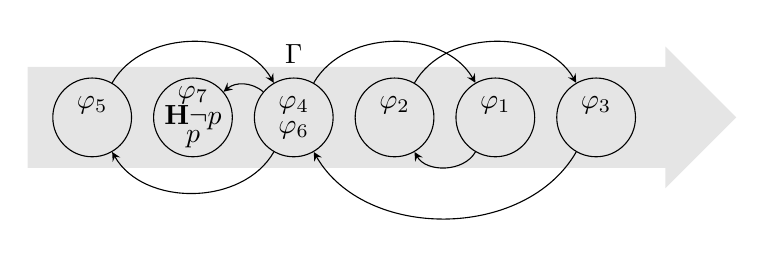
\begin{tikzpicture}[>=stealth, scale=.8,
world/.style={minimum size=1cm, draw=black, circle},
intension/.style={fill=black, fill opacity=.1},
altrel/.style={->},
bejaras/.style={blue}]

%%%%%%%%%%% SETTINGS %%%%%%%%%%%%%%%
\pgfmathsetmacro{\HorDist}{1.6}
\pgfmathtruncatemacro{\Darab}{6}
\pgfmathtruncatemacro{\EdgeAngle}{60}

%%%%%%%%%%% SZÁMOLANDÓK %%%%%%%%%%%%%%%
\pgfmathtruncatemacro{\nyilhossz}{\Darab+3}

\foreach \i in {1,2, ..., \Darab}
{\node[world](v\i) at (\HorDist*\i,0){};}

\node[single arrow,
fill=black,
fill opacity=.1,
single arrow head extend=.05cm,
minimum height=\nyilhossz cm,
minimum width=1.8cm,
single arrow head indent=0cm] at (1+.5*\HorDist*\Darab,0){};

\node at (3*\HorDist ,1) {$\Gamma$};

\draw[->] (v3) edge[in = 180-\EdgeAngle, out=\EdgeAngle](v5);
\node at (5*\HorDist ,0.2) {$\varphi_1$};
\pause %%%%%%%%%%%% PAUSE %%%%%%%%%%%%%
\draw[->] (v5) edge[in = -\EdgeAngle, out=-180+\EdgeAngle](v4);
\node at (4*\HorDist ,0.2) {$\varphi_2$};
\pause %%%%%%%%%%%% PAUSE %%%%%%%%%%%%%
\draw[->] (v4) edge[in = 180-\EdgeAngle, out=\EdgeAngle](v6);
\node at (6*\HorDist ,0.2) {$\varphi_3$};
\pause %%%%%%%%%%%% PAUSE %%%%%%%%%%%%%
\draw[->] (v6) edge[in = -\EdgeAngle, out=-180+\EdgeAngle](v3);
\node at (3*\HorDist ,0.2) {$\varphi_4$};
\pause %%%%%%%%%%%% PAUSE %%%%%%%%%%%%%
\draw[->] (v3) edge[in = -\EdgeAngle, out=-180+\EdgeAngle](v1);
\node at (1*\HorDist ,0.2) {$\varphi_5$};
\pause %%%%%%%%%%%% PAUSE %%%%%%%%%%%%%
\draw[->] (v1) edge[in = 180-\EdgeAngle, out=\EdgeAngle](v3);
\node at (3*\HorDist ,-0.2) {$\varphi_6$};
\pause %%%%%%%%%%%% PAUSE %%%%%%%%%%%%%
\draw[->] (v3) edge[in =-20+\EdgeAngle, out=200-\EdgeAngle](v2);
\node at (2*\HorDist ,0.35) {$\varphi_7$};
\pause %%%%%%%%%%%% PAUSE %%%%%%%%%%%%%
\node at (2*\HorDist ,-.35) {$p$};
\node at (2*\HorDist ,0) {$\mathbf H\lnot p$};

\end{tikzpicture}\]

\vspace{-2em}
We willl focus on those \cemph{maximally $\mathbf O$-consistent} theories that \cemph{can prove their innocence easily} and \cemph{are in the company of easily provable innocents}. To do so, however, we will start with a different notion, which will mean the same for maximally $\mathbf {O}$-consistent sets.
\end{frame}

\begin{frame}[t]
	\frametitle{IRR-theories}
\scriptsize

\bemph{Intuitively,} $\Gamma$ is an \cemph{IRR-theory} iff
%\[
$\Gamma \derives[O] p \land \mathbf H \lnot p \textup{ for some $p\in \mathrm {At}$,}$
%\]
and
\[\lrule[l]
         {  \textup{For all $p\in \mathrm{At}$ not occurring in $\varphi_1, \dots , \varphi_n$,}
         \\ \Gamma \derives[O]\mathrm{L}_1 (\varphi_1 \lthen \mathrm{L}_2 (\varphi_2 \lthen \dots \lthen \mathrm{L}_{n-1}(\varphi_{n-1}\lthen \mathrm L_n(\varphi_n\lthen (\lnot (p \land \mathbf H\lnot p))) )\dots ))}
         {\Gamma \derives[O] \mathrm{L}_1 (\varphi_1 \lthen \mathrm{L}_2 (\varphi_2 \lthen \dots \lthen \mathrm{L}_{n-1}(\varphi_{n-1}\lthen \mathrm L_n(\varphi_n \lthen \bot))\dots ))}
\]
where $\mathrm{L}_i\in \{\Box, \FB, \PB\}$ for all $i\leq n$. 
\bigskip

\bemph{Precisely,}
\[\begin{tomb}{rcl}
   {}[\varnothing;\varnothing](\#)&\defegy& \#,
\\ {}[\langle\mathrm L,\vec{\mathrm L} \rangle;\langle \varphi, \vec\varphi \rangle](\#)&\defegy &\mathrm L ( \varphi \lthen [\vec{\mathrm L} ; \vec\varphi](\#))\textup{ where }\mathrm L \in \{\Box, \FB, \PB \}
\end{tomb}\]
and ${}[\vec{\mathrm L};\vec \varphi] (\varphi)\defegy {}[\vec{\mathrm L};\vec \varphi] ( {\#} / \varphi)$. Then $\Gamma$ is IRR iff
\[\lrule[l]
         {  \textup{For all $p\in \mathrm{At}$ not occurring in $\vec \varphi$,}
         \\ \Gamma \derives[O] [\vec{\mathrm L};\vec \varphi] (\lnot (p \land \mathbf H \lnot  p))}
         {  \Gamma \derives[O] [\vec{\mathrm L};\vec \varphi] (\bot)}\]
where $\vec{\mathrm L}$ is an $n$-tuple over $\{\Box, \FB, \PB\}$.

%\dzsa{Proposition}
%\derives[O] $\psi \lthen [\vec{\mathrm L};\vec \varphi] (\varphi) \liff ([\vec{\mathrm L};\psi \land \vec \varphi] \lor [\vec{\mathrm L};\vec \varphi] )$

\end{frame}

%%%%%%%%%%%%%%%%%%%%%%%%%%%%%%%%%%%%%%%%%%%%%%%%%%%%%%%%%%%%%%%%%%%%%%%%%%%%%%%%%%%%%%%%%%%%%%
\begin{frame}[t]
\frametitle{\bemph{(IRRExt)}}
\scriptsize

%\begin{itemize}
%\item Any \cemph{finite} consistent theory can be extended to a maximally consistent IRR-theory.
A consistent theory in which \cemph{an infinite number of atomic propositions do not occur}, can be extended to a consistent IRR theory.
%\end{itemize}
\medskip
\hrule
\medskip
\dzsa{Proof}% \bemph{Idea: We put an evidence for irreflexivity in $\Gamma$ (we can do so, since there are atomic sentences to which $\Gamma$ is indifferent) by hand, and we continue with the standard Lindenbaum's lemma in a way to ensure that the resulting set will be an IRR theory.}

So let $\Gamma$ be a consistent theory described above, and let $p$ an atom not occurring in $\Gamma$.

Let $\Sigma_0\defegy \Gamma\cup \{p \land \PB \lnot p\}$. This is consistent, for if
\[\begin{array}{rcll}
   \Gamma \cup \{ p \land \mathbf H \lnot p \} & \derives & \bot & \magyi{ind.ass.}
\\ \Gamma  & \derives & \lnot (p \land \mathbf H \lnot p ) & \magyi{Ded.thm.}
\\ \exists \Gamma_{\mathrm{finite}}\supseteq \Gamma  & \derives & \lnot (p \land \mathbf H \lnot p ) & \magyi{def.of $\derives$}
\\ & \derives & \bigwedge \Gamma_{\mathrm{finite}} \lthen \lnot (p \land \mathbf H \lnot  p ) & \magyi{def.of $\derives$}
\\ & \derives & (p \land \mathbf H \lnot p ) \lthen \lnot \bigwedge \Gamma_{\mathrm{finite}} & \magyi{contraposition}
\\ & \derives & \lnot \bigwedge \Gamma_{\mathrm{finite}} & \textup{\tiny\cemph{IRR-rule}}
\\ \Gamma_{\mathrm{finite}}& \derives & \bot & \magyi{ded.thm}
\\ \Gamma& \derives & \bot & \textup{QED}\end{array}\]
%and that contradicts to the assumption that $\Gamma$ was consistent. %\bemph{So let us prove that this rule is valid indeed!}
\[\tiny
\usetikzlibrary[shapes.arrows]
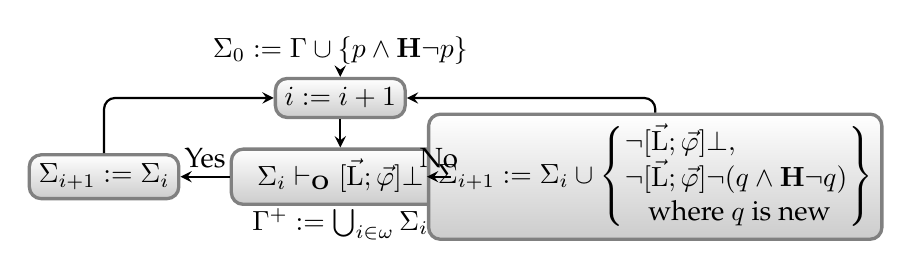
\begin{tikzpicture}[scale=1,>=stealth,
allapot/.style={ rectangle,rounded corners=1.5mm,very thick,draw=black!50,top color=white,bottom color=black!20,
}]
\pgfmathsetmacro{\magassag}{-1}
\node(0) at (0,.45){};
\node[allapot](i) at (0,0){$i:=i+1$};
\node[allapot](test) at (0,\magassag){\begin{tabular}{c}
  $\Sigma_i \vdash_{\mathbf{O}} {}[\vec{\mathrm L}; \vec \varphi] \bot$
\end{tabular}};
\node[allapot](yes-case) at (-3,\magassag){$\Sigma_{i+1} := \Sigma_i$};
\node[allapot](no-case) at (4,\magassag)
{$\Sigma_{i+1} :=
\Sigma_i\cup
\left\{ \arraycolsep=.1mm\begin{array}{l}
   \lnot [\vec{\mathrm L}; \vec \varphi]\bot ,
        \\{}
        \lnot [\vec{\mathrm L}; \vec \varphi] \lnot (q\land \mathbf H \lnot q)
        \\{} \hfill \textup{ where $q$ is new}
   \end{array}
   \right\}$};
\begin{scope}[->, thick, rounded corners=4pt]
\draw (0)--(i);
\draw (i)--(test);
\draw (test)--(no-case) node[pos=.5, above, inner sep=1mm]{No};
\draw (test)--(yes-case)node[pos=.5, above, inner sep=1mm]{Yes};
\draw (yes-case)|-(i);
\draw (no-case)|-(i);
\end{scope}
\node at (0,0.6) {$\Sigma_0: = \Gamma \cup \{p\land \mathbf H\lnot p\}$};
\node at (0,-1.6) {$%\displaystyle
\Gamma^+:= \bigcup_{i\in \omega} \Sigma_i$};
\end{tikzpicture}
\]\end{frame}

%%%%%%%%%%%%%%%%%%%%%%%%%%%%%%%%%%%%%%%%%%%%%%%%%%%%%%%%%%%%%%%%%%%%%%%%%%%%%%%%%%%%%%%%%%%%%%%%%%%%%%%%%%%%%%%%%%
\begin{frame}
\frametitle{\bemph{(IRRLin)}}
\[\textup{Every consistent IRR set is extendable to a maximally consistent IRR set.}\]
\hrule
\[\tiny
\usetikzlibrary[shapes.arrows]
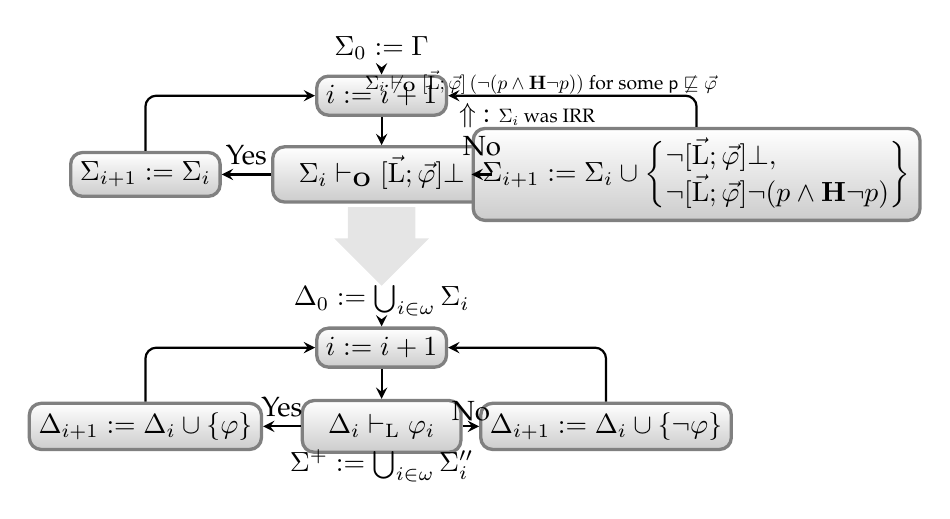
\begin{tikzpicture}[scale=1,>=stealth,
allapot/.style={ rectangle,rounded corners=1.5mm,very thick,draw=black!50,top color=white,bottom color=black!20,
}]

\pgfmathsetmacro{\magassag}{-1}

\node(0) at (0,.45){};
\node[allapot](i) at (0,0){$i:=i+1$};

\node[allapot](test) at (0,\magassag){\begin{tabular}{c}
  $\Sigma_i \vdash_{\mathbf{O}} {}[\vec{\mathrm L}; \vec \varphi] \bot$
\end{tabular}};

\node[allapot](yes-case) at (-3,\magassag){$\Sigma_{i+1} := \Sigma_i$};

\node[allapot](no-case) at (4,\magassag)
{$\Sigma_{i+1} :=
\Sigma_i\cup
\left\{ \arraycolsep=.1mm\begin{array}{l}
   \lnot [\vec{\mathrm L}; \vec \varphi]\bot ,
        \\{}
        \lnot [\vec{\mathrm L}; \vec \varphi] \lnot (p\land \mathbf H \lnot p)
   \end{array}
   \right\}$};

\begin{scope}[->, thick, rounded corners=4pt]
\draw (0)--(i);
\draw (i)--(test);
\draw (test)--(no-case) node[pos=.5, above, inner sep=1mm]{\begin{tabular}{c} \hspace{1.5cm}\scalebox{.7}{$\Sigma_i \not \vdash_{\mathbf{O}} [\vec{\mathrm L}; \vec \varphi]\,( \lnot (p \land \mathbf H \lnot p))$ for some $\mathsf p\not\sqsubseteq \vec \varphi$} \\ \hspace{1.15cm}$\Uparrow$ : \scalebox{.7}{$\Sigma_i$ was IRR}\\ No \end{tabular}};
\draw (test)--(yes-case)node[pos=.5, above, inner sep=1mm]{Yes};
\draw (yes-case)|-(i);
\draw (no-case)|-(i);
\end{scope}



\begin{scope}[yshift=-3.2cm]
\node at (0,.6) {$\Delta_0 := \bigcup_{i\in \omega} \Sigma_i$ };
\node(0) at (0,.45){};
\node[allapot](i) at (0,0){$i:=i+1$};

\node[allapot](test) at (0,\magassag){\begin{tabular}{c}
  $\Delta_i\vdash_{\mathrm{L}} \varphi_i$
\end{tabular}};

\node[allapot](yes-case) at (-3,\magassag){$\Delta_{i+1} := \Delta_i\cup \{\varphi\}$};

\node[allapot](no-case) at (2.85,\magassag){$\Delta_{i+1} := \Delta_i\cup \{ \lnot \varphi\}$};

\begin{scope}[->, thick, rounded corners=4pt]
\draw (0)--(i);
\draw (i)--(test);
\draw (test)--(no-case) node[pos=.5, above, inner sep=.5mm]{No};
\draw (test)--(yes-case)node[pos=.5, above, inner sep=1mm]{Yes};
\draw (yes-case)|-(i);
\draw (no-case)|-(i);
\end{scope}
\node at (0,-1.5){$\Sigma^+ := \bigcup_{i\in \omega} \Sigma''_i$ };
\end{scope}


\node[single arrow, rotate=-90,
fill=black,
fill opacity=.1,
single arrow head extend=.05cm,
minimum height=1 cm,
minimum width=1.2cm,
single arrow head indent=0cm] at (0,-1.7) {};

\node at (0,0.6) {$\Sigma_0: = \Gamma $};
\end{tikzpicture}
\]
\end{frame}

%%%%%%%%%%%%%%%%%%%%%%%%%%%%%%%%%%%%%%%%%%%%%%%%%%%%%%%%%%%%%%%%%%%%%%%%%%%%%%%%%%%%%%%%%%%%%%%

\begin{frame}[t]
	\frametitle{\bemph{$(\mathrm L^-)$}}
For $\mathrm{L}\in \{\Box, \FB, \PB\}$,
\[\Gamma \textup{ is IRR } \Longrightarrow \mathrm{L}^-(\Gamma) \textup{ is IRR }\]
\hrule
\medskip

\dzsa{Proof}
Let $\varphi \sqsubseteq \vec\psi$ denote that $\varphi$ is a subformula of an element of $\vec \psi$:
\[\begin{tomb}{lrcll}
     \forallp {p \not\sqsubseteq \vec\varphi}
   & \mathrm{L}^- (\Gamma)
   & \derives[O]
   & {}[\vec {\mathrm{L}}; \vec \varphi ](\lnot (p \land \mathbf H\lnot p))
   & \magyi{assumption}
\\   \forallp {p \not\sqsubseteq \vec\varphi}
   & \mathrm{L}^- (\Gamma)
   & \derives[O]
   & {}\top \lthen [\vec {\mathrm{L}}; \vec \varphi ](\lnot (p \land \mathbf H\lnot p))
   & \magyi{PC}
\\   \forallp {p \not\sqsubseteq \vec\varphi}
   & \Gamma
   & \derives[O]
   & \mathrm{L}(\top \lthen [\vec {\mathrm{L}}; \vec \varphi ](\lnot (p \land \mathbf H\lnot p)))
   & \magyi{$\mathrm L^-$-thing}
\\   \forallp {p \not\sqsubseteq \vec\varphi}
   & \Gamma
   & \derives[O]
   & [\langle \mathrm L, \vec {\mathrm{L}}\rangle ; \langle \top , \vec \varphi \rangle ](\lnot (p \land \mathbf H\lnot p))
   & \magyi{def.of templates}
\\ & \Gamma
   & \derives[O]
   & [\langle \mathrm L, \vec {\mathrm{L}}\rangle ; \langle \top , \vec \varphi \rangle ](\bot)
   & \magyi{$\Gamma$ is IRR}
\\ & \Gamma
   & \derives[O]
   & \mathrm{L}(\top \lthen [\vec {\mathrm{L}}; \vec \varphi ](\bot))
   & \magyi{def.of templates}
\\ & \mathrm L^-(\Gamma)
   & \derives[O]
   & \top \lthen [\vec {\mathrm{L}}; \vec \varphi ](\bot)
   & \magyi{$\mathrm L^-$-thing}
\\ & \mathrm L^-(\Gamma)
   & \derives[O]
   & [\vec {\mathrm{L}}; \vec \varphi ](\bot)
   & \magyi{PC}
\end{tomb}\]
\end{frame}

\begin{frame}[t]
	\frametitle{\bemph{(FE)}}
For $\mathrm{L}\in \{\Box, \FB, \PB\}$,
\[\Gamma \textup{ is IRR } \Longrightarrow \Gamma \cup \{\varphi\} \textup{ is IRR }\]
\hrule
\medskip
\scriptsize

\dzsa{Proof}
Let $\varphi \sqsubseteq \vec\psi$ denote that $\varphi$ is a subformula of an element of $\vec \psi$:
\[\begin{tomb}{lrcll}
     \forallp {p \not\sqsubseteq \vec\varphi}
   & \Gamma \cup \{\varphi\}
   & \derives[O]
   & {}[\vec {\mathrm{L}}; \vec \varphi ](\lnot (p \land \mathbf H\lnot p))
\hfill \magyi{assumption}
\\   \forallp {p \not\sqsubseteq \vec\varphi}
   & \Gamma \cup \{\varphi\}
   & \derives[O]
   & {}[\langle \mathrm L_1, \mathrm L_2, \dots , \mathrm L_n\rangle; \langle \varphi_1, \varphi_2, \dots , \varphi_n\rangle ](\lnot (p \land \mathbf H\lnot p))
\\&&& \hfill  \magyi{focusing on the inside of $\vec \varphi$ and $\vec{\mathrm L}$}
\\   \forallp {p \not\sqsubseteq \vec\varphi}
   & \Gamma \cup \{\varphi\}
   & \derives[O]
   & \mathrm L_1( \varphi_1 \lthen {}[\langle\mathrm L_2, \dots , \mathrm L_n\rangle; \langle \varphi _2, \dots , \varphi_n\rangle ](\lnot (p \land \mathbf H\lnot p)))
\\&&& \hfill  \magyi{def.of templates}
\\   \forallp {p \not\sqsubseteq \vec\varphi}
   & \mathrm L_1^-(\Gamma \cup \{\varphi\})
   & \derives[O]
   & \varphi_1 \lthen {}[\langle\mathrm L_2, \dots , \mathrm L_n\rangle; \langle \varphi _2, \dots , \varphi_n\rangle ](\lnot (p \land \mathbf H\lnot p))
\\&&& \hfill  \magyi{$\mathrm L_1$-thing}
\\   \forallp {p \not\sqsubseteq \vec\varphi}
   & \mathrm L_1^-(\Gamma) \cup \mathrm L_1^-(\{\varphi\})
   & \derives[O]
   & \varphi_1 \lthen {}[\langle\mathrm L_2, \dots , \mathrm L_n\rangle; \langle \varphi _2, \dots , \varphi_n\rangle ](\lnot (p \land \mathbf H\lnot p))
\\&&& \hfill  \magyi{$\mathrm L_1^-$ distributes over $\cup$.}
\end{tomb}\]
\end{frame}

\begin{frame}[t]
	\frametitle{\bemph{(FE)}}
\scriptsize
\vspace{-1.5em}
$\qquad \qquad \qquad $ \cemph{Now if $\varphi$ is of form $\mathrm L_1 \psi$, then}
\[\hspace{-.7cm}\begin{tomb}{lrcll}
   \forallp {p \not\sqsubseteq \vec\varphi}
   & \mathrm L_1^-(\Gamma) \cup \mathrm L_1^-(\{\mathrm L_1 \psi \})
   & \derives[O]
   & \varphi_1 \lthen {}[\langle\mathrm L_2, \dots , \mathrm L_n\rangle; \langle \varphi _2, \dots , \varphi_n\rangle ](\lnot (p \land \mathbf H\lnot p))
\\&&& \hfill \magyi{$\mathrm L_1^-$ distributes over $\cup$.}
\\   \forallp {p \not\sqsubseteq \vec\varphi}
   & \mathrm L_1^-(\Gamma) \cup \{\psi\}
   & \derives[O]
   & \varphi_1 \lthen {}[\langle\mathrm L_2, \dots , \mathrm L_n\rangle; \langle \varphi _2, \dots , \varphi_n\rangle ](\lnot (p \land \mathbf H\lnot p))
\\[-1em]&&& \hfill \magyi{def.of $\mathrm L_1^-$}
\\   \forallp {p \not\sqsubseteq \vec\varphi}
   & \mathrm L_1^-(\Gamma)
   & \derives[O]
   & (\psi\land \varphi_1) \lthen {}[\langle\mathrm L_2, \dots , \mathrm L_n\rangle; \langle \varphi _2, \dots , \varphi_n\rangle ](\lnot (p \land \mathbf H\lnot p))
\\&&& \hfill \magyi{ded.thm}
\\   \forallp {p \not\sqsubseteq \vec\varphi}
   & \Gamma
   & \derives[O]
   & \mathrm L_1 ((\psi\land \varphi_1 )\lthen {}[\langle\mathrm L_2, \dots , \mathrm L_n\rangle; \langle \varphi _2, \dots , \varphi_n\rangle ](\lnot (p \land \mathbf H\lnot p)))
\\&&& \hfill \magyi{$\mathrm L_1$-thing}
\\   \forallp {p \not\sqsubseteq \vec\varphi}
   & \Gamma
   & \derives[O]
   & [\langle\mathrm L_1, \mathrm L_2, \dots , \mathrm L_n\rangle; \langle \psi\land \varphi_1 , \varphi _2, \dots , \varphi_n\rangle ](\lnot (p \land \mathbf H\lnot p))
\\&&& \hfill \magyi{def.of templates}
%\\   \forallp {p \not\sqsubseteq \vec\varphi}
%   & \Gamma
%   & \derives[O]
%   & [\vec {\mathrm L}; \langle \psi\land \varphi_1 , \varphi _2, \dots , \varphi_n\rangle ](\lnot (p \land \mathbf H\lnot p))
%\\&&& \hfill \magyi{abbreviating}
\\ & \Gamma
   & \derives[O]
   & [\langle\mathrm L_1, \mathrm L_2, \dots , \mathrm L_n\rangle; \langle \psi\land \varphi_1 , \varphi _2, \dots , \varphi_n\rangle ](\bot)
\\[-1em]&&& \hfill \magyi{$\Gamma$ is IRR}
\\ & \Gamma
   & \derives[O]
   & \mathrm L_1 ( (\psi \land \varphi_1) \lthen [\langle\mathrm L_2, \dots , \mathrm L_n\rangle; \langle \varphi _2, \dots , \varphi_n\rangle ](\bot))
\\&&& \hfill \magyi{def.of templates}
\\ & \mathrm L_1^-(\Gamma)
   & \derives[O]
   &  (\psi \land \varphi_1) \lthen [\langle\mathrm L_2, \dots , \mathrm L_n\rangle; \langle \varphi _2, \dots , \varphi_n\rangle ](\bot)
\\[-1em]&&& \hfill \magyi{$\mathrm L_1$-thing}
\\ & \mathrm L_1^-(\Gamma) \cup \{\psi\}
   & \derives[O]
   &  \varphi_1 \lthen [\langle\mathrm L_2, \dots , \mathrm L_n\rangle; \langle \varphi _2, \dots , \varphi_n\rangle ](\bot)
\\[-1em]&&& \hfill \magyi{ded.thm}
\\ & \mathrm L_1^-(\Gamma) \cup \mathrm L_1^-(\{\mathrm L_1 \psi\})
   & \derives[O]
   &  \varphi_1 \lthen [\langle\mathrm L_2, \dots , \mathrm L_n\rangle; \langle \varphi _2, \dots , \varphi_n\rangle ](\bot)
\\[-1em]&&& \hfill \magyi{ded.thm}
\\ & \mathrm L_1^-(\Gamma) \cup \mathrm L_1(\{\varphi\})
   & \derives[O]
   &  \varphi_1 \lthen [\langle\mathrm L_2, \dots , \mathrm L_n\rangle; \langle \varphi _2, \dots , \varphi_n\rangle ](\bot)
\\[-1em]&&& \hfill \magyi{def.of $\mathrm L_1^-$}
\\ & \mathrm L_1^-(\Gamma\cup \{\varphi\})
   & \derives[O]
   &  \varphi_1 \lthen [\langle\mathrm L_2, \dots , \mathrm L_n\rangle; \langle \varphi _2, \dots , \varphi_n\rangle ](\bot)
\\[-1em]&&& \hfill \magyi{$\mathrm L_1^-$ distributes over $\cup$}
\\ & \Gamma\cup \{\varphi\}
   & \derives[O]
   & \mathrm L_1( \varphi_1 \lthen [\langle\mathrm L_2, \dots , \mathrm L_n\rangle; \langle \varphi _2, \dots , \varphi_n\rangle ](\bot))
\\[-1em]&&& \hfill \magyi{$\mathrm L_1$-thing}
\\ & \Gamma\cup \{\psi\}
   & \derives[O]
   & [\langle\mathrm L_1, \mathrm L_2, \dots , \mathrm L_n\rangle; \langle \varphi_1 , \varphi _2, \dots , \varphi_n\rangle ](\bot)
\\[-1em]&&& \hfill \magyi{def.of template}
\\ & \Gamma\cup \{\psi\}
   & \derives[O]
   & [\vec {\mathrm L}\rangle; \langle \vec\varphi\rangle ](\bot)
\\[-1em]&&& \hfill \magyi{vector-notation}
\end{tomb}\]

\end{frame}

\begin{frame}[t]
	\frametitle{\bemph{(FE)}}
\scriptsize
\vspace{-1.5em}
$\qquad \qquad \qquad $ \cemph{Now if $\varphi$ is NOT of form $\mathrm L_1 \psi$, then}
\[\hspace{-.7cm}\begin{tomb}{lrcll}
   \forallp {p \not\sqsubseteq \vec\varphi}
   & \mathrm L_1^-(\Gamma) \cup \mathrm L_1^-(\{\varphi\})
   & \derives[O]
   & \varphi_1 \lthen {}[\langle\mathrm L_2, \dots , \mathrm L_n\rangle; \langle \varphi _2, \dots , \varphi_n\rangle ](\lnot (p \land \mathbf H\lnot p))
\\&&& \hfill \magyi{$\mathrm L_1^-$ distributes over $\cup$.}
\\   \forallp {p \not\sqsubseteq \vec\varphi}
   & \mathrm L_1^-(\Gamma) \cup \varnothing
   & \derives[O]
   & \varphi_1 \lthen {}[\langle\mathrm L_2, \dots , \mathrm L_n\rangle; \langle \varphi _2, \dots , \varphi_n\rangle ](\lnot (p \land \mathbf H\lnot p))
\\&&& \hfill \magyi{def.of $\mathrm L_1^-$}
\\   \forallp {p \not\sqsubseteq \vec\varphi}
   & \mathrm L_1^-(\Gamma)
   & \derives[O]
   & \varphi_1 \lthen {}[\langle\mathrm L_2, \dots , \mathrm L_n\rangle; \langle \varphi _2, \dots , \varphi_n\rangle ](\lnot (p \land \mathbf H\lnot p))
\\   \forallp {p \not\sqsubseteq \vec\varphi}
   & \Gamma
   & \derives[O]
   & \mathrm L_1 (\varphi_1 \lthen {}[\langle\mathrm L_2, \dots , \mathrm L_n\rangle; \langle \varphi _2, \dots , \varphi_n\rangle ](\lnot (p \land \mathbf H\lnot p)))
\\&&& \hfill \magyi{$\mathrm L_1$-thing}
\\   \forallp {p \not\sqsubseteq \vec\varphi}
   & \Gamma
   & \derives[O]
   & [\langle\mathrm L_1, \mathrm L_2, \dots , \mathrm L_n\rangle; \langle \varphi_1 , \varphi _2, \dots , \varphi_n\rangle ](\lnot (p \land \mathbf H\lnot p))
\\&&& \hfill \magyi{def.of templates}
%\\   \forallp {p \not\sqsubseteq \vec\varphi}
%   & \Gamma
%   & \derives[O]
%   & [\vec {\mathrm L}; \langle \psi\land \varphi_1 , \varphi _2, \dots , \varphi_n\rangle ](\lnot (p \land \mathbf H\lnot p))
%\\&&& \hfill \magyi{abbreviating}
\\ & \Gamma
   & \derives[O]
   & [\langle\mathrm L_1, \mathrm L_2, \dots , \mathrm L_n\rangle; \langle \varphi_1 , \varphi _2, \dots , \varphi_n\rangle ](\bot)
\\[-1em]&&& \hfill \magyi{$\Gamma$ is IRR}
\\ & \Gamma
   & \derives[O]
   & \mathrm L_1 ( \varphi_1 \lthen [\langle\mathrm L_2, \dots , \mathrm L_n\rangle; \langle \varphi _2, \dots , \varphi_n\rangle ](\bot))
\\&&& \hfill \magyi{def.of templates}
\\ & \mathrm L_1^-(\Gamma)
   & \derives[O]
   &  \varphi_1 \lthen [\langle\mathrm L_2, \dots , \mathrm L_n\rangle; \langle \varphi _2, \dots , \varphi_n\rangle ](\bot)
\\[-1em]&&& \hfill \magyi{$\mathrm L_1$-thing}
\\ & \mathrm L_1^-(\Gamma) \cup \{\varnothing\}
   & \derives[O]
   & \varphi_1 \lthen [\langle\mathrm L_2, \dots , \mathrm L_n\rangle; \langle \varphi _2, \dots , \varphi_n\rangle ](\bot)
\\[-1em]&&& \hfill \magyi{ded.thm}
%\\ & \mathrm L_1^-(\Gamma) \cup \mathrm L_1^-(\{\varphi\})
%   & \derives[O]
%   & \varphi_1 \lthen [\langle\mathrm L_2, \dots , \mathrm L_n\rangle; \langle \varphi _2, \dots , \varphi_n\rangle ](\bot)
%\\[-1em]&&& \hfill \magyi{}
\\ & \mathrm L_1^-(\Gamma) \cup \mathrm L_1^-(\{\varphi\})
   & \derives[O]
   &  \varphi_1 \lthen [\langle\mathrm L_2, \dots , \mathrm L_n\rangle; \langle \varphi _2, \dots , \varphi_n\rangle ](\bot)
\\[-1em]&&& \hfill \magyi{def.of $\mathrm L_1^-$}
\\ & \mathrm L_1^-(\Gamma\cup \{\varphi\})
   & \derives[O]
   &  \varphi_1 \lthen [\langle\mathrm L_2, \dots , \mathrm L_n\rangle; \langle \varphi _2, \dots , \varphi_n\rangle ](\bot)
\\[-1em]&&& \hfill \magyi{$\mathrm L_1^-$ distributes\dots}
\\ & \Gamma\cup \{\varphi\}
   & \derives[O]
   & \mathrm L_1( \varphi_1 \lthen [\langle\mathrm L_2, \dots , \mathrm L_n\rangle; \langle \varphi _2, \dots , \varphi_n\rangle ](\bot))
\\[-1em]&&& \hfill \magyi{$\mathrm L_1$-thing}
\\ & \Gamma\cup \{\psi\}
   & \derives[O]
   & [\langle\mathrm L_1, \mathrm L_2, \dots , \mathrm L_n\rangle; \langle \varphi_1 , \varphi _2, \dots , \varphi_n\rangle ](\bot)
\\[-1em]&&& \hfill \magyi{def.of template}
\\ & \Gamma\cup \{\psi\}
   & \derives[O]
   & [\vec {\mathrm L}\rangle; \langle \vec\varphi\rangle ](\bot)
\\[-1em]&&& \hfill \magyi{vector-notation}
\end{tomb}\]

\end{frame}


%%%%%%%%%%%%%%%%%%%%%%%%%%%%%%%%%%%%%%%%%%%%%%%%%%%%%%%%%%%%%%%%%%%%%%%%%%%%%%%%%%%%%%%%%%%%%%%%%%%%%

\szakasz[Irr. can. submodel]{Irreflexive canonical submodel}

\begin{frame}
\frametitle{Canonical Kamp model}

\[\mathfrak M_{\mathbf O} \defegy \left( W_{\mathbf O}, <_{\mathbf O}, \equiv_{\mathbf O}, V_{\mathbf O}\right)   \]
where
\begin{itemize}
\item $W_{\mathbf O} \defegy \{\Gamma \, :\, \textup{$ \Gamma$  is a maximally $\mathbf O$-consistent \cemph{IRR-theory}} \}$,
\item $\Gamma <_{\mathbf O}\Gamma'$ iff $\FB^-(\Gamma )\subseteq  \Gamma'$ \bemph{Remember that these are equivalent:
\\ \hfill $\begin{tomb}{rcl}
          \FB^-(\Gamma )&\subseteq & \Gamma'
\\ \Gamma &\supseteq & \FD^+(\Gamma')
\\ \Gamma &\supseteq & \PB^-(\Gamma')
\\ \PD^+(\Gamma)&\subseteq & \Gamma'
\end{tomb}$}
\item $\Gamma \equiv_{\mathbf O}\Gamma'$ iff $\Box^-(\Gamma )\subseteq \Gamma'$, \bemph{Similarly:
$\begin{tomb}{rcl}
          \Box^-(\Gamma )&\subseteq & \Gamma'
\\ \Gamma &\supseteq & \Diamond^+(\Gamma')
\end{tomb}$}
\item $\Gamma \in V_{\mathbf O}(p) \defekv p\in \Gamma$.
\end{itemize}
\end{frame}

%%%%%%%%%%%%%%%%%%%%%%%%%%%%%%%%%%%%%%%%%%%%%%%%%%%%%%%%%%%%%%%%%%%%%%%%%%%%%%%%%%%%%%%%%%%%%%%%%%%5

\begin{frame}
\frametitle{\bemph{(Ex)}}
Let $\mathrm M$ denote the dual pair of $\mathrm L$. 
\[\mathrm M \varphi \in \Gamma  \mathrel{\cemph{\Longrightarrow}} \existsin {\Gamma'}{\cemph{W_\mathbf O}} \big[\Gamma' \supseteq \mathrm{L}^-(\Gamma) \textup{ and } \varphi \in \Gamma' \big]\]

\hrule
\medskip

Since $\Gamma$ is IRR, so are $\mathrm L^-(\Gamma)$ and $\mathrm L^-(\Gamma) \cup\{\varphi\}$, by (\bemph{$\mathrm L^-$}) and \bemph{(FE)}. The latter is consistent by the standard argumentation:
%\dzsa{Lemma} If $\Gamma$ is a max.con. set, then
%\[ \mathrm M \varphi \in \Gamma \quad \Longrightarrow\quad \mathrm L^-(\Gamma) \cup\{\varphi\}\not \derives[O] \bot\]
%\dzsa{proof}
\bemph{\tiny\[ \begin{tomb}{rcll}
   \mathrm L^- (\Gamma) \cup \{\varphi\}&\vdash_{\mathbf O}&\bot &\textup{indirect assumption}
\\ \mathrm L^- (\Gamma)&\vdash_{\mathbf O}& \lnot \varphi &\textup{Deduction theorem}
\\ \exists \vec \chi &\vdash_{\mathbf O}& \lnot \varphi &\textup{def.of $\mathrm L^- (\Gamma)\vdash_{\mathbf O}$}
\\ &\vdash_{\mathbf O}& \bigwedge\vec\chi \lthen \lnot \varphi &\textup{def.of $\vdash_{\mathbf O}$}
\\ &\vdash_{\mathbf O}& \mathrm L \bigwedge\vec\chi \lthen \mathrm L \lnot \varphi &\textup{Lemmon}
\\ &\vdash_{\mathbf O}& \bigwedge\mathrm L\vec\chi \lthen \mathrm L \lnot \varphi &\textup{A-axiom}
\\ \bigwedge\mathrm L\vec\chi &\vdash_{\mathbf O}& \mathrm L \lnot \varphi & \textup{def.of $\vdash_{\mathbf O}$}
\\ \Gamma &\vdash_{\mathbf O}& \mathrm L \lnot \varphi &\chi\in \mathrm L^-(\Gamma) \Leftrightarrow \mathrm L \chi\in \Gamma
\\ \Gamma &\vdash_{\mathbf O}& \lnot \FD\varphi &\textup{Duality}
\\ \Gamma \cup \{ \FD\varphi \}&\vdash_{\mathbf O}& \bot &\textup{Deduction theorem}
\\ \Gamma &\vdash_{\mathbf O}& \bot &\textup{by the assumption $\FD \varphi \in \Gamma$. QED}
\end{tomb}\]}
So we can extend $\mathrm L^-(\Gamma) \cup\{\varphi\}$ by \bemph{(IRRLin)} into a maximally $\mathbf O$-consistent IRR theory, and we are ready.

\end{frame}
%%%%%%%%%%%%%%%%%%%%%%%%%%%%%%%%%%%%%%%%% NEXT SLIDE %%%%%%%%%%%%%%%%%%%%%%%%%%%%%%%%%%%%%%%%555555
\begin{frame}
\frametitle{Summary}
\begin{itemize}
\item The Truth Lemma goes through by our new existence lemma.
\item $V_\mathbf{O}$ is a Kamp-valuation by the axiom of the unpreventability of past.
\[ (UPP)\qquad \varphi \lthen \Box \varphi \textup{ where $\FD$ does not occur in $\varphi$}\]
\item $<_{\mathbf O}$ is irreflexive by construction (all our canonical worlds are IRR theories).
\item $<_{\mathbf O}$ is transitive and non-branching by the canonicity of 4 and .3.
\item $\equiv_{\mathbf O}$ is reflexive, transitive and symmetric by the canonicity of T, 4 and B.
\item $\Gamma \equiv_{\mathbf O} \Delta \lthen \Gamma\not <_{\mathbf O}\Delta $ comes from (UPP) and from the construction:
There is a $p\land \PB \lnot p\in \Delta$, by UPP, $\Box (p\land \PB \lnot p)\in \Delta$, by def of $\equiv_{\mathbf O}$, and the symmetry of it, $p\land \PB \lnot p\in \Gamma$.
But $\Gamma <_{\mathbf O}\Delta$ would mean that $\PB^-(\Delta)\subseteq \Gamma$, so $\lnot p\in \Gamma$ which causes a contradiction.
\item $(w \equiv v \land w'<w ) \lthen \existsp {v'<v} \;w'\equiv v'$ -- We prove this on the next slide
\item $\forallp{w,v}\existsp{w'<w}\existsp {v'<v} \;w\equiv v$ As in usual, we can take the generated submodels to validate this.
\item \cemph{$\forallp{w,v} (w \equiv v \land w\neq v) \existsp{w'>w}\forallp {v'>v} \;w'\not\equiv v'$} that is not true, we will have to suffer with this later
\end{itemize}
\end{frame}
%%%%%%%%%%%%%%%%%%%%%%%%%%%%%%%%%%%%%%%%%%%%%%%%%%%%%%%%%%%%%%%%%%%%%%%%%%%%%%%%%%%%%%%%%%%%%%%%%%%5

\begin{frame}
\[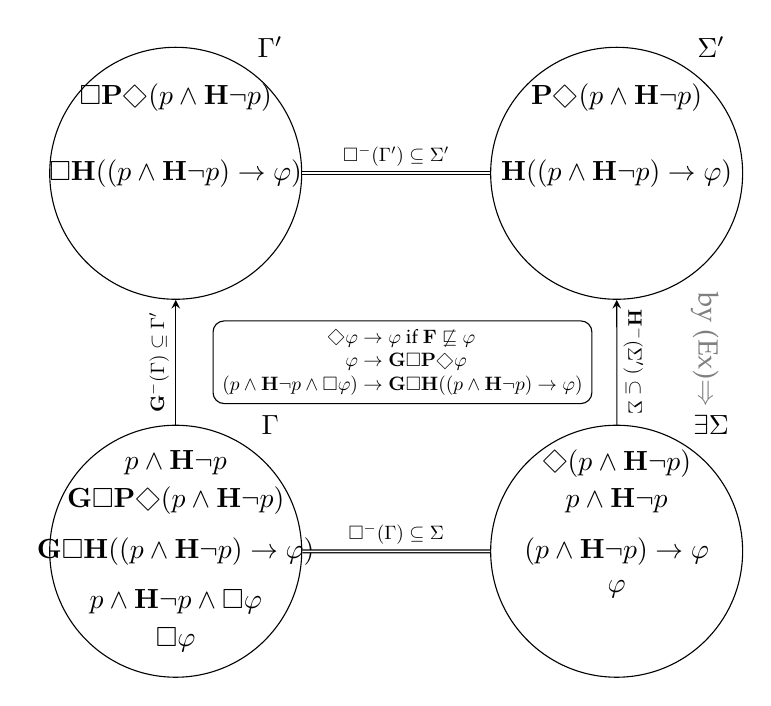
\begin{tikzpicture}[world/.style={inner sep=.4mm, fill=black, circle},set/.style={minimum size=3.2cm, draw=black, circle},>=stealth, scale=1.6]
\node[set](G') at (0,0) {};
\node[set](S') at (3.5,0) {};
\node[set](G) at (0,-3) {};
\draw[->]  (G) -- (G')node[sloped, midway, scale=.7, above]{$\mathbf G^-(\Gamma)\subseteq \Gamma'$};
\draw[double]  (G') -- (S') node[sloped, midway, scale=.7, above]{$\Box^-(\Gamma')\subseteq \Sigma'$};
\node at (0.75,1) {$\Gamma'$};
\node at (0.75,-2) {$\Gamma$};
\node at (4.25,1) {$\Sigma'$};
\node[draw=black, rounded corners, scale=.7] at (1.8,-1.5) {$\arraycolsep =.5mm\begin{array} {rcl}
\Diamond \varphi &\to& \varphi \textup{ if }\mathbf F \not \sqsubseteq \varphi
\\ \varphi &\to& \mathbf G \Box \mathbf P \Diamond \varphi
\\ (p\land \mathbf H \lnot p \land \Box \varphi )&\to& \mathbf G \Box \mathbf H ((p\land \mathbf H \lnot p )\to \varphi)
\end{array}$};
\node at (0,-2.3) {$p\land \mathbf H \lnot p$};
\pause %%%%%%%%%%%%%%%%%% --- PAUSE --- %%%%%%%%%%%%%%%%%%
\node at (0,-2.6) {$\mathbf G \Box \mathbf P \Diamond (p\land \mathbf H \lnot p )$};
\pause %%%%%%%%%%%%%%%%%% --- PAUSE --- %%%%%%%%%%%%%%%%%%
\node at (0,0.6) {$\Box \mathbf P \Diamond(p\land \mathbf H \lnot p )$};
\pause %%%%%%%%%%%%%%%%%% --- PAUSE --- %%%%%%%%%%%%%%%%%%
\node at (3.5,0.6) {$\mathbf P \Diamond(p\land \mathbf H \lnot p )$};
\pause %%%%%%%%%%%%%%%%%% --- PAUSE --- %%%%%%%%%%%%%%%%%%
\node[rotate=-90, opacity=.5] at (4.2,-1.4) {by ({Ex})$\Rightarrow $};
\node [set](S) at (3.5,-3) {};
\draw[->]  (S) -- (S')node[sloped, midway, scale=.7, above]{$\mathbf H^-(\Sigma')\subseteq \Sigma$};
\node at (4.25,-2) {$\exists \Sigma$};
\node at (3.5,-2.3) {$\Diamond (p\land \mathbf H \lnot p )$};
\pause %%%%%%%%%%%%%%%%%% --- PAUSE --- %%%%%%%%%%%%%%%%%%
\node at (3.5,-2.6) {$p\land \mathbf H \lnot p $};
\pause %%%%%%%%%%%%%%%%%% --- PAUSE --- %%%%%%%%%%%%%%%%%%
%%%%%%%%%%%%%%%%%%%%%%%%%%%%%%%%%%%%
%%%%%%%%%%%%% MÁSODIK RÉSZ %%%%%%%%%%%%%%
%%%%%%%%%%%%%%%%%%%%%%%%%%%%%%%%%%%%
\node at (0,-3.7) {$\Box \varphi$};
\pause %%%%%%%%%%%%%%%%%% --- PAUSE --- %%%%%%%%%%%%%%%%%%
\node at (0,-3.4) {$p\land \mathbf H\lnot p \land \Box \varphi$};
\pause %%%%%%%%%%%%%%%%%% --- PAUSE --- %%%%%%%%%%%%%%%%%%
\node at (0,-3) {$\mathbf G \Box \mathbf H ((p\land \mathbf H\lnot p) \to \varphi)$};
\pause %%%%%%%%%%%%%%%%%% --- PAUSE --- %%%%%%%%%%%%%%%%%%
\node at (0,0) {$\Box \mathbf H ((p\land \mathbf H\lnot p) \to \varphi)$};
\pause %%%%%%%%%%%%%%%%%% --- PAUSE --- %%%%%%%%%%%%%%%%%%
\node at (3.5,0) {$\mathbf H ((p\land \mathbf H\lnot p) \to \varphi)$};
\pause %%%%%%%%%%%%%%%%%% --- PAUSE --- %%%%%%%%%%%%%%%%%%
\node at (3.5,-3) {$(p\land \mathbf H\lnot p) \to \varphi$};
\pause %%%%%%%%%%%%%%%%%% --- PAUSE --- %%%%%%%%%%%%%%%%%%
\node at (3.5,-3.3) {$\varphi$};
\pause %%%%%%%%%%%%%%%%%% --- PAUSE --- %%%%%%%%%%%%%%%%%%
\draw[double]  (G) -- (S) node[sloped, midway, scale=.7, above]{$\Box^-(\Gamma)\subseteq \Sigma$};
\end{tikzpicture}\]
\end{frame}

\szakasz[Maximalizing Histories]{Maximalizing Histories}


\end{document}

